\documentclass[11pt]{article}

    % Packages this paper needs
    \usepackage{fullpage, hyperref,bbm,amssymb,amsfonts,amsthm}
    \usepackage[noend]{algorithmic}
    \usepackage{algorithm}
    \usepackage{setspace}
    \usepackage{cleveref}
    \usepackage{color}
    \usepackage{latexsym}
    \usepackage{verbatim}
    \usepackage{graphics}
    \usepackage{graphicx}
    \usepackage{multicol}
    
    
    
    \newcommand{\<}{\langle}
    \renewcommand{\>}{\rangle}
    \newcommand{\C}{\mathbb{C}}
    \newcommand{\cA}{\mathcal{A}}
    \newcommand{\cB}{\mathcal{B}}
    \newcommand{\cE}{\mathcal{E}}
    \newcommand{\cF}{\mathcal{F}}
    \newcommand{\cH}{\mathcal{H}}
    \newcommand{\cK}{\mathcal{K}}
    \newcommand{\cM}{\mathcal{M}}
    \newcommand{\cR}{\mathcal{R}}
    \newcommand{\cU}{\mathcal{U}}
    \newcommand{\cV}{\mathcal{V}}
    \newcommand{\cZ}{\mathcal{Z}}
    \newcommand{\E}{\mathrm{\mathbf{E}}}
    \newcommand{\Var}{\mathrm{\mathbf{Var}}}
    \newcommand{\EE}[1]{\E\left(#1\right)}
    \newcommand{\VV}[1]{\Var\left(#1\right)}
    \newcommand{\s}{\mathrm{span}}
    \newcommand{\R}{\mathbb{R}}
    
    \renewcommand{\sim}{\mathrm{sim}}
    \renewcommand{\prec}{\mathrm{prec}}
    \newcommand{\fail}{\mathrm{fail}}
    \newcommand{\median}{\mathrm{median}}
    \newcommand{\anc}{\mathrm{anc}}
    
    \newcommand{\kets}[1]{| #1 \rangle}                 % small ket vector
    \newcommand{\bras}[1]{\langle #1 |}                 % small bra vector
    \newcommand{\braket}[2]{\langle #1 | #2 \rangle}         % <x|y>
    \newcommand{\ii}{\mathbb{I}}
    % the I with two vertical lines
    \newcommand{\norms}[1]{\big\| #1\big\|}          % norm
    \newcommand{\ep}{\epsilon}
    
    % the I with two vertical lines
    \newcommand{\twonorm}[1]{\left\| #1\right\|_2}        % norm
    \newcommand{\inftynorm}[1]{\left\| #1\right\|_\infty}
    \newtheorem{fact}{Fact}
    
    % epsilon
    \newcommand{\tr}{\mathrm{tr}}
    %\newcommand{\qed}{\hfill $\square$}
    \newtheorem{definition}{Definition}
    \newtheorem{theorem}{Theorem}
    \newtheorem{lemma}{Lemma}
    \newtheorem{proposition}{Proposition}
    \newtheorem{cor}{Corollary}
    \newtheorem{remark}{Remark}
    \newtheorem*{problem}{Problem}
    
    
    % style
    \theoremstyle{definition}
    \begin{document}
    \title{Problem Set 1 for CS 540/495}
     \author{Michaela Laden, Caleb Perry, Tucker Mogren, Kyle Saunders}				
    \maketitle
    %%%%%%%%%
    \begin{abstract}  %
    %%%%%%%%%
    This report will summarize how Simulated Annealing can be used to find the best solutions to the Vehicle Routing Problem as it is discussed by Ibrahim Hassan Osman in \textit{Metastrategy simulated annealing and Tabu search algorithms for the vehicle routing problem}. 
    \end{abstract}
    
    %%%%%%%%%%%%
    \section{Introduction} 
    There are many cases where simulated annealing would be a valid generic algorithm to use in order to solve a specific problem. An example problem that benefits from the use of simulated annealing is the Vehicle Routing Problem. This problem is very similar to the common "Traveling Salesman" problem and explores how Simulated Annealing can be used to find the minimum costs between a set of delivery routes, where the originating and terminating location is a central terminal. There are many different variations of the Vehicle Routing Problem. Some variations focus on the use of different vehicle applications (EX: deliveries, tours, etc). This is a widely studied problem and using Simulated Annealing in order to find the best result for this problem has proven to be successful. 
    
    %
    %%%%%%%%%%%%
    
    
    %%%%%%%%%%%%%%%
    \section{The Background} 
    %%%%%%%%%%%%%%%
    \begin{problem}
    The Vehicle Routing Problem is a problem that asks what is the best route for a fleet of vehicles to take in order to deliver to a certain set of customers within a given time period.
    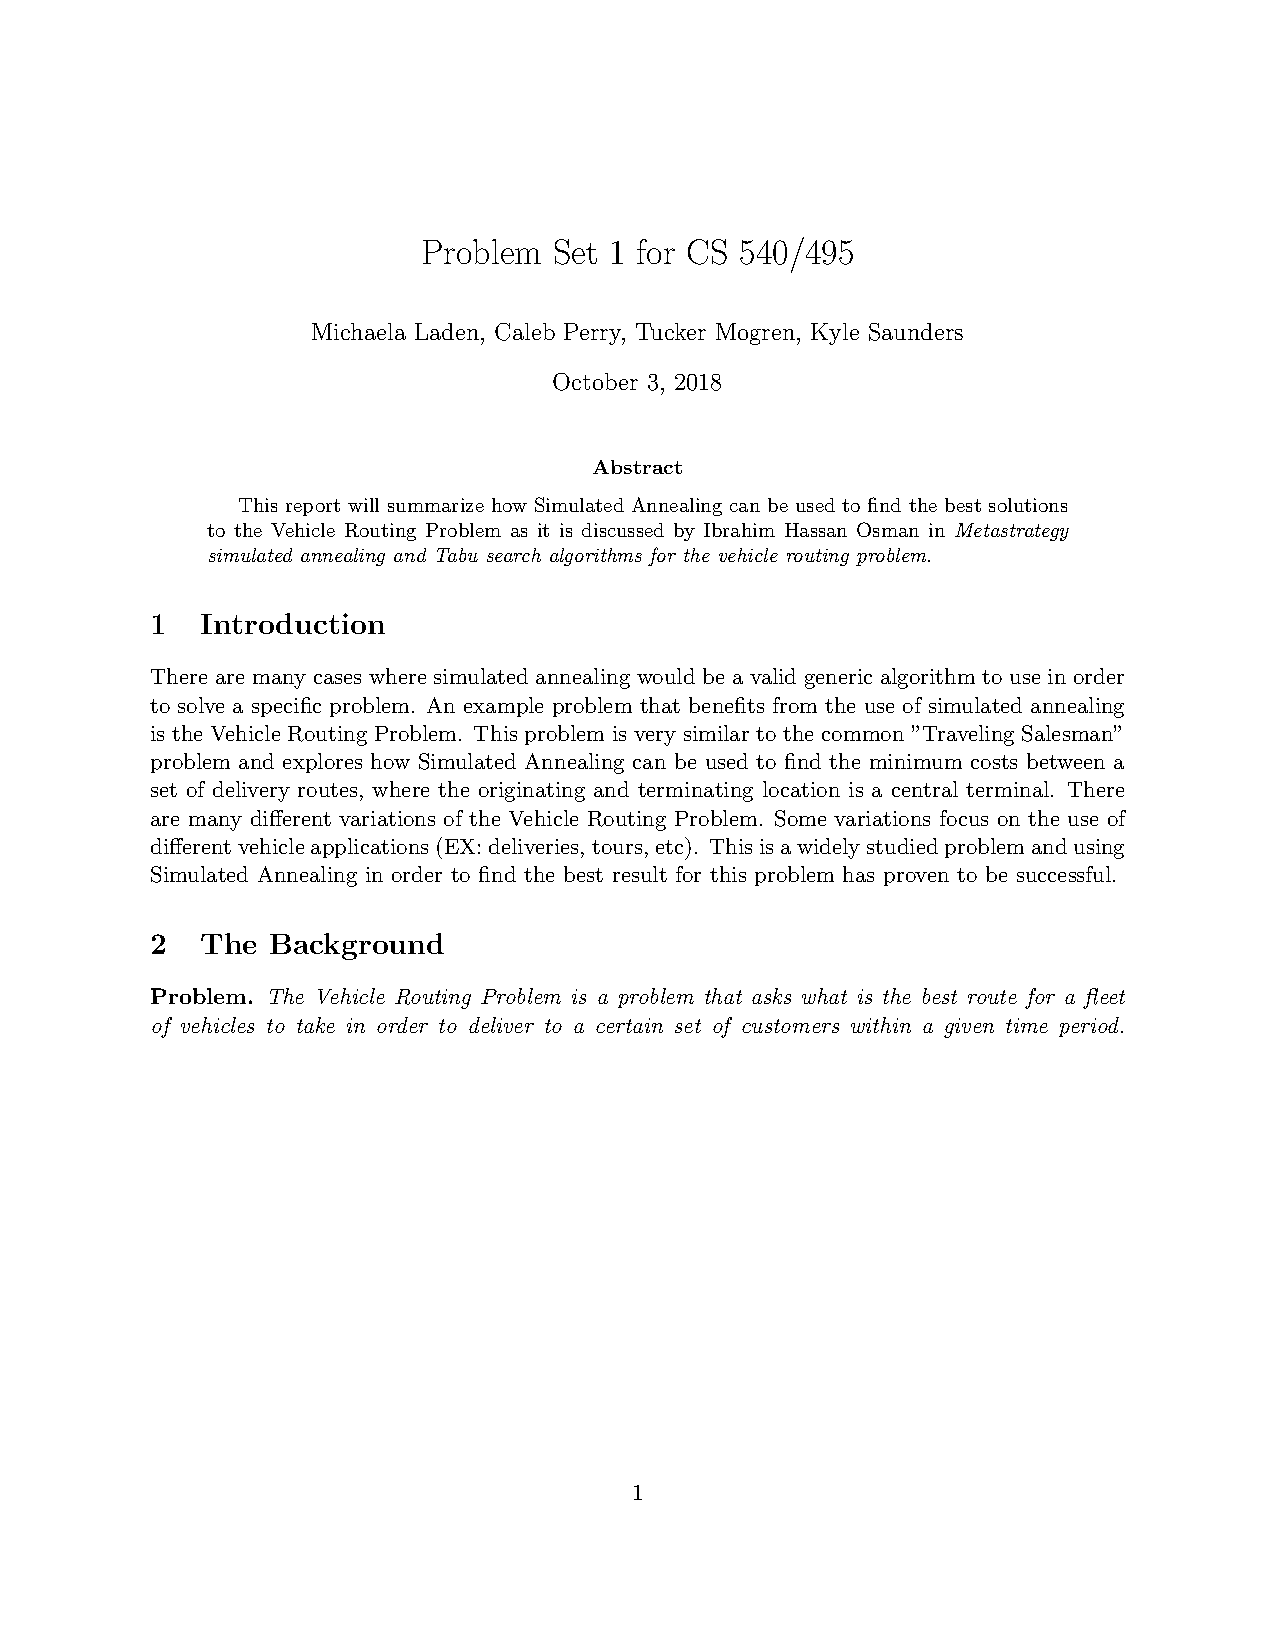
\includegraphics[width=\textwidth]{AI.PNG}\\
    n = the number of customers\\
    N = the set of Customers, N = \{1,..........n\}\\
    $q_i$ = The demand of the customer i $\epsilon$ N (i = 0 denotes the depot, $q_0$ = 0)\\
    $g_i$ = The service time of customer i $\epsilon$ N ($g_0$ = 0)\\
    ${c_i}_j$ = The travel time (distance) between customers i and j, ${c_i}_j$ = ${c_i}_j$ $\forall_i$, j $\epsilon$ N (${c_i}_j$ = $\infty$, $\forall$i $\epsilon$ N )\\
    v = The number of vehicles, which is a \textit{decision} variable in our problem;\\
    V = The set of vehicles, V = \{1,.......,v\};\\
    Q = The vehicle capacity;\\
    $R_p$ = The set of customers serviced by vehicle p;\\
    C($R_p$) = The cost (length) of the optimal traveling salesmen tour $\pi_p$ over the customers in 
    $R_p$$\cup$\{0\}. This cost includes the travel times (${c_i}_j$) and the service times ($\delta_i$);\\
    L = The prespecified upper bound on the maximum tour length;\\
    S = The feasible solution which is defined as S = \{$R_1$, ......, $R_v$\};\\
    C(S) = The total sum of each individual tour length C($R_p$) for all P $\epsilon$ V\\\\\\
    Our goal is to find the best solution  that minimizes the total travel length and time.
    \end{problem}
    \subsection{Diagrams}
    \includegraphics[width=\textwidth]{AI2.PNG}\\
    The above diagram shows two different kinds of routes the driver could take. Tour 1 shows a route where the driver starts at the Central terminal and makes all the proper stops, only returning to the terminal when the route is complete. The second tour, Tour 2, shows a route the driver would have to take if they had to return to the terminal number times during the route in order to restock packages.\\
    \includegraphics[width=\textwidth]{AI3.PNG}\\
    %%%%%%%%%%
    
    \section{The Algorithm}
    For the Vehicle Routing Problem (VPR) the specific algorithm used is the non-monotonic Simulated Annealing cooling schedule. This cooling schedule requires specifications such as, starting and final temperatures, decrement rule for updating the temperature $T_k$ after each iteration k, update rule for temperature reset variables $T_{r}$ after the system freezes, stopping criterion R, which is the total number of temperature resets to be performed after the best solution was found. This method uses 1-interchange mechanism to generate neighboring solutions where the neighborhoods are then searched in the indicated order. The algorithm performs a single iteration at each temperature. \\ 
    
    \subsection{The Procedure}
    The following procedure is a hybrid of Simulated Annealing and Tabu Search ideas. This specific method differs from the local search descent methods because in other methods sigma is fixed to an order of \{1,....,v\}. For this method the search for a given pair ($R_{p}, R_{q}$) is systematic for all potential customer moves as in the descent methods. It has become evident that using the non-monotonic cooling schedule with an ordered search outperforms other simulated annealing algorithms.\\
    \noindent\rule{17cm}{0.4pt}\\
    \\\textbf{Step 1}: Generate an initial heuristic solution S by the savings method.\\
    \\\textbf{Step 2}: Initialize the cooling schedule parameters: 
    perform a test cycle of search over the neighborhood \textit{N(S)} of the initial solution without performing the exchanges in order to obtain the largest and smallest $\Delta_{max}$ change in objective function values, and an estimate of the total number of feasible exchanges \textit{Nfeas}.
    Set {$T_s$=$\Delta_{max}$, $T_f$=$\Delta_{min}$, $T_r=T_s$, $\alpha$ = n $\times$ Nfeas, $\gamma$ = n, R=3, $s_b$=S and k=1}\\
    \\\textbf{Step 3}: Select a solution S'$\in N_1$(S) in ordered search and compute $\Delta$ = \textit{C(S')-C(S)} according to cost evaluation procedure.\\
    \\\textbf{Step 4}: If {($\Delta \leq 0$ or $\Delta > 0$ and e$^{-\Delta/T_k}$ $\geq \theta$, where $\theta$ is a uniform random parameter 0 $< \theta <1$}
    \textbf{Then} accept the new solution \textit{S'}, compute $\Delta$ according to cost procedure(b), set \textit{S=S'}
        if \textit{$C(S')<C(S_b)$}, then \textit{$S_b=S'$} and \textit{$T_b = T_k$}, the temperature at which the best solution is found;
        \textbf{otherwise} return \textit{S}.\\
    \\\textbf{Step 5}: Update temperatures according to:\\ 
    \\\textit{Normal decrement rule:}\\
    \\$T_{k}$=$\frac{T_{k}}{1+\beta_{k}T_{k}}$, where $\beta_{k}$=$\frac{T_{s}-T_{f}}{(\alpha + \gamma \sqrt{k}) T_{s}T_{f}}$;\\
    \\or \textit{Occasional increment rule:} If a cycle of search is completed without accepting any 1-interchange move, update as\\
    \\ $T_{r}$= $max \bigg\{\frac{T_{r}}{2}, T_{b}\bigg\}$ and set $T_{k}=T_{r}$.\\
    \\Set \textit{k=k+1}.
    \\\textbf{Step 6}: \textbf{Stop} if the stopping criterion is met(R resets were performed sin \textit{$S_{b}$} was found), report the best solution \textit{$S_{b}$} and computation time. \\
    \textbf{Otherwise}, go to step 3.
    \\
    %%%%%%%%%%%%%%%%%%%%%%%%%%%%%%%%%%%%%%%%%%%%%%%%%%%%%%%%%%%%%%%%%%%%%%
    \section{The Complexity \& Discussion}
    %%%%%%%%%%%%%%%%%%%%%%%%%%%%%%%%%%%%%%%%%%%%%%%%%%%%%%%%%%%%%%%%%%%%%%
    The gain in complexity, theoretically or heuristically such as where it excels. Furthermore, can you describe where this can be further \textbf{improved} or any related work that can be benefit from this line of research? 
    
    
    As stated above, this problem very closes mirrors the Traveling Salesman problem and its solution can be directly implemented when derived from the Traveling Salesman. A situation like this requires thousands, if not millions of iterations in order to find the best, most efficient solution. 
    
    
    The Vehicle Routing Problem, takes into account capacity, and distance restrictions that are involved in the process of designing and discovering minimum delivery costs. It is understood that one vehicle will be assigned to one route and that the vehicle that is assigned to said route will not have its predetermined capacity exceeded. 
    
    The complexity of the simulated annealing implementation used in the case described in the book (the VRP problem or "Vehicle Routing Problem") has very a few slight differences from a plain SA implementation that generate more complexity than a normal SA solution. For example, in their implementation of the Simulated Annealing algorithm they also opted to include a way to intelligently guide the Simulated Annealing algorithm toward a next step that is more then likely going to be an improvement from the last. But, this is not always the case as they also made sure to keep the logic that would choose a step to take that would result in some loses in fitness in the hopes that the (in this case) global minima would be found. They did this by implementing a tabu search algorithm alongside their simulated annealing algorithm that would remember when going down a certain branch has led to non optimal results. This allowed only branches that were considered by the algorithm to be 'non-dead' branches to be discovered and subsequently explored.
    
    In theory, this type of implementation has the potential to be much more costly per iteration than a normal SA search but it also has the benefit of completing its search in fewer iterations when compared to a normal SA search. However, in their actual application of said algorithm, they incurred some widely varying results as a result of this hybrid algorithm.
    
    Of all algorithms tested, the SA/TS hybrid algorithm found some of the best and some of the worst results taking a total average time per computational cycle of 4909 seconds; making it four times slower than the best algorithm tested in this study. Their conclusion contained sentiments that such an algorithm is very useful when used on a 'medium' or 'large' sized problem as the incurred overhead of the TS is only worth it when many iterations are required. The best results this algorithm gave was a solution using only 163 cars which was down 4 from the previously held record of 167 cars. Their Tabu Search + First Best Admissible algorithm found resulting solutions that were close but not quite as good as the best solution found by the SA + TS search but did so with much computational time.
    
    This algorithm could be improved or tweaked in a few different ways. The algorithm used in the paper used an arbitrary temperature control system and as a result might not have had as good results as they might have gotten had they tested a pure SA solution with differing temperature control systems to find one that best suit the problem used in the study. Another way this algorithm could have been optimized is if they used a Tabu Search that doesn't remember every bad branch but instead just the bad ones around where the algorithm's current search location is. This is called a Short Term Memory Tabu Search and is listed in the book as a type of tabu search looked into as part of their research but they did not use it in their SA based solution. If they had used a short term memory solution then the time it would take for the tabu search to 'green light' the SA algorithm to take the next step would not grow exponentially with every iteration  like it does in the study. Instead, the algorithm would only save the last 'n' dead branches found and would drop dead branches that it is not likely to visit again.
    
    This type of algorithm would be great if used as an implementation of the traveling salesman problem as its tabu search elements combined with the SA algorithm can lead to very efficient results if given enough time to compute said results.
    
    %%%%%%%%%%%%%%%%%%%%%%%%%%%%%%%%%%%%%%%%%%%%%%%%%%%%%%%%%%%%%%%%%%%%%%
    \begin{thebibliography}{9}
    \bibitem{Metastrategy simulated annealing and Tabu search
    algorithms for the vehicle routing problem} 
    Ibrahim Hassan Osman,
    Metastrategy simulated annealing and Tabu search
    algorithms for the vehicle routing problem.
    \end{thebibliography}
    
    \end{document}
    %%%%%%%%%%%%%%%%%%%%%%%%%%%%%%%%%%%%%%%%%%%%%%%%%%%%%%%%%%%%%%%%%%%%%%%%%%%%%%%%%
    